\documentclass[12pt, twoside]{article}
\usepackage[letterpaper, margin=1in, headsep=0.5in]{geometry}
\usepackage[english]{babel}
\usepackage[utf8]{inputenc}
\usepackage{amsmath}
\usepackage{amsfonts}
\usepackage{amssymb}
\usepackage{tikz}
\usetikzlibrary{quotes, angles}
\usepackage{graphicx}
%\usepackage{pgfplots}
%\pgfplotsset{width=10cm,compat=1.9}
%\usepgfplotslibrary{statistics}
%\usepackage{pgfplotstable}
%\usepackage{tkz-fct}
%\usepackage{venndiagram}

\usepackage{fancyhdr}
\pagestyle{fancy}
\fancyhf{}
\renewcommand{\headrulewidth}{0pt} % disable the underline of the header

\fancyhead[RE]{\thepage}
\fancyhead[RO]{\thepage \\ Name: \hspace{3cm}}
\fancyhead[L]{BECA / Dr. Huson / Geometry 10th Grade\\* Unit 3: Volume and angle bisectors  \\ 
3 October 2019}

\begin{document}
  \subsubsection*{3.2 Homework: Segment \& Area Calculations}
  \begin{enumerate}
  
  \item Complete the construction of the bisector of the given angle. 
  \vspace{3cm}
    \begin{center}
    \begin{tikzpicture}
      \draw [<->, thick] (50:7)--(0,0)--(9,0);
      %\draw [fill] (0,0) circle [radius=0.05] node[below]{$A$};
      %\draw [fill] (5,0) circle [radius=0.05] node[below]{$B$};
    \end{tikzpicture}
    \end{center} \vspace{4cm}

  \item Given the rectangle $ABCD$ shown below, with $BC=5 \frac{3}{7}$. If the area of the rectangle is 76, find $AB$.
    \begin{flushleft}
    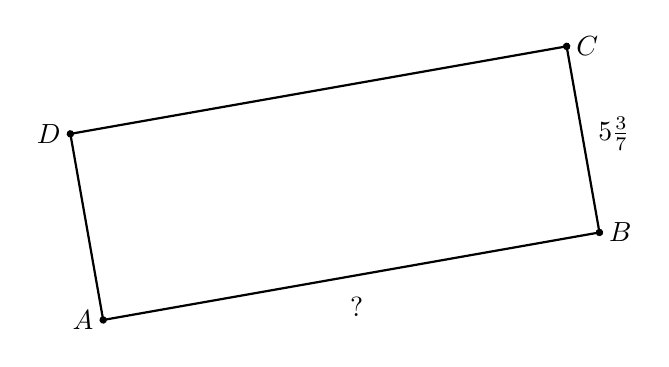
\begin{tikzpicture}[scale=0.8, rotate=10]
      \draw [-, thick] (0,0)--(8,0)--(8,3)--(0,3)--cycle;
      \draw [fill] (0,0) circle [radius=0.05] node[left]{$A$};
      \draw [fill] (8,0) circle [radius=0.05] node[right]{$B$};
      \draw [fill] (8,3) circle [radius=0.05] node[right]{$C$};
      \draw [fill] (0,3) circle [radius=0.05] node[left]{$D$};
      \node at (8.5, 1.5){$5 \frac{3}{7}$};
      \node at (4, -0.5){?};
    \end{tikzpicture}
    \end{flushleft}
    \vspace{1.5cm}

\newpage

  \item The area of a square is 144 square feet. 
    \begin{enumerate}
      \item Find the length of the side of the square $s$. \vspace{2cm}
      \item Find the perimeter of the square.
    \end{enumerate} \vspace{2cm}

  \item Given $\overleftrightarrow{FG}$ as shown on the number line, with $F=-1.7$ and $G=6.1$. \\[20pt] % Midpoint
  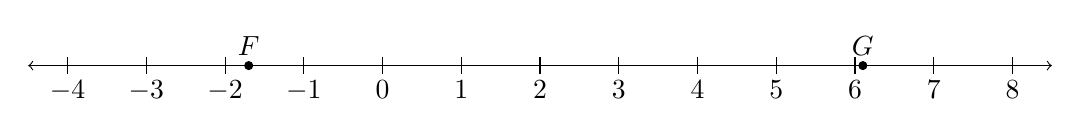
\begin{tikzpicture}
    \draw [<->] (-4.5,0)--(8.5,0);
    \foreach \x in {-4,...,8} %2 leading for diff!=1
      \draw[shift={(\x,0)},color=black] (0pt,-3pt) -- (0pt,3pt) node[below=5pt]  {$\x$};
      \draw [fill] (-1.7,0) circle [radius=0.05] node[above] {$F$};
      \draw [fill] (6.1,0) circle [radius=0.05] node[above] {$G$};
  \end{tikzpicture}\\[5pt]
  The point $H$ is the bisector of $\overline{FG}$. Find the value of $H$, and mark and label it on the numberline $\overleftrightarrow{FG}$ above. 
  \vspace{3cm}

  \item Given that $m\angle 2= 5x+30$ and $m\angle 4=7x-10$ as shown in the diagram, find $m\angle 2$.
  \begin{flushright}
  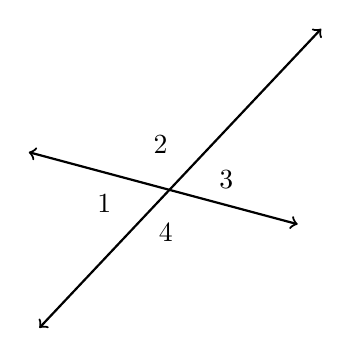
\begin{tikzpicture}[scale=0.5, rotate=30]
    \draw [<->, thick] (0,-1.5)--(10,1.5);
    \draw [<->, thick] (2,2.5)--(7,-2.5);
    \node at (3,.4){1};
    \node at (6,-.6){3};
    \node at (5,1){2};
    \node at (4,-1){4};
  \end{tikzpicture}
  \end{flushright}

\end{enumerate}
\end{document}
